\documentclass[12pt]{article}
\usepackage[utf8]{inputenc}
\usepackage[margin=1in]{geometry}
\usepackage{amsmath}
\usepackage{amssymb}
\usepackage{graphicx}
\usepackage{enumerate}
\graphicspath{ {./images/} }

\author{Neelu Saraswatibhatla (srns2)}
\title{Operating Systems Supervision 3}
\date{\vspace{-5ex}}

\begin{document}

\maketitle

\section{Example Sheet 4}

\begin{enumerate}
    \item The basic access control scheme is to have read, write, and execute access to each file. More advanced access control policies are implemented by allowing these permissions to be set by user, group, and world.
    \item \begin{enumerate}
        \item As seen in the diagram below, the filesystem contains a boot block and one or more partitions. Each partition has a superblock, an inode table, and data blocks. The boot blochk contains the location of each filesystem (partition). The superblock contains the number of blocks and free blocks in the filesystem and other bookkeeping information. Free inodes and blocks are located together with allocated ones, and a list is kept of the free ones.\\
        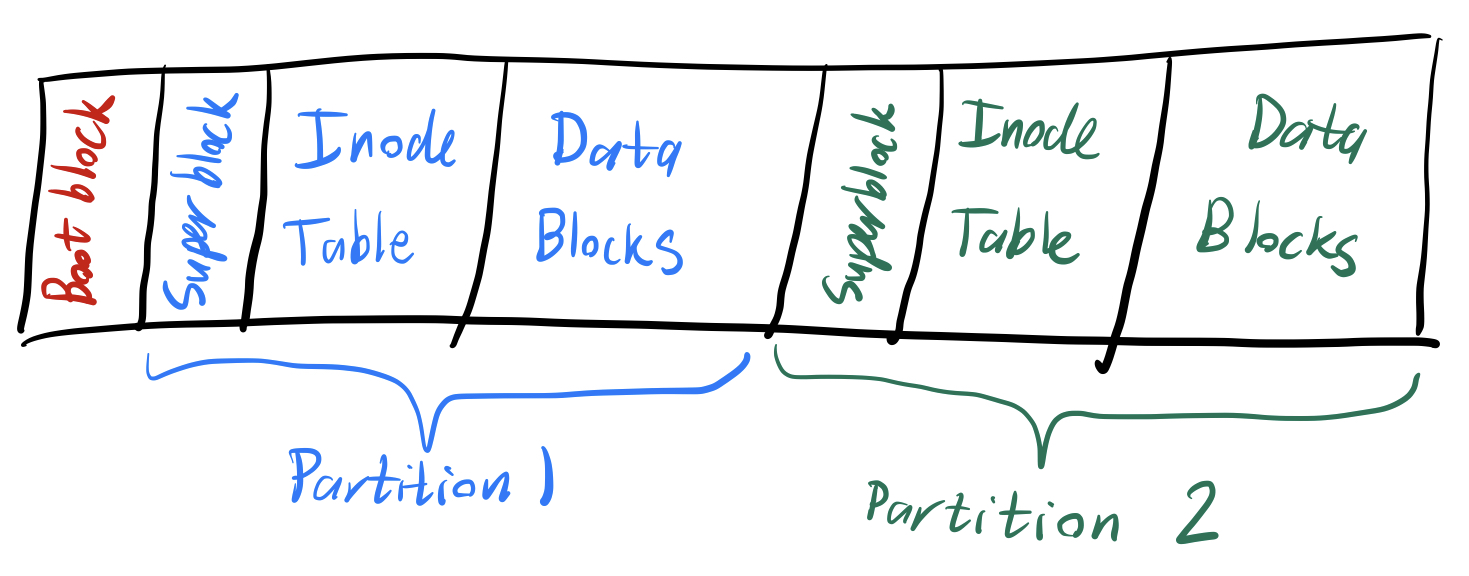
\includegraphics[scale=0.25]{2a.jpg}
        \item An inode contains various things \begin{itemize}
            \item Bookkeeping information such as type, size, etc. It is important to note that the inode does NOT contain the file name or permissions, as these are stored in the directory rather than in the inode.
            \item 12 direct blocks which point directly to data.
            \item A single indirect block which points to 512 direct blocks, each of which point to data.
            \item A double indirect block which points to 512 single indirect blocks.
            \item A triple indirect block which points to 512 double indirect blocks.
        \end{itemize}
        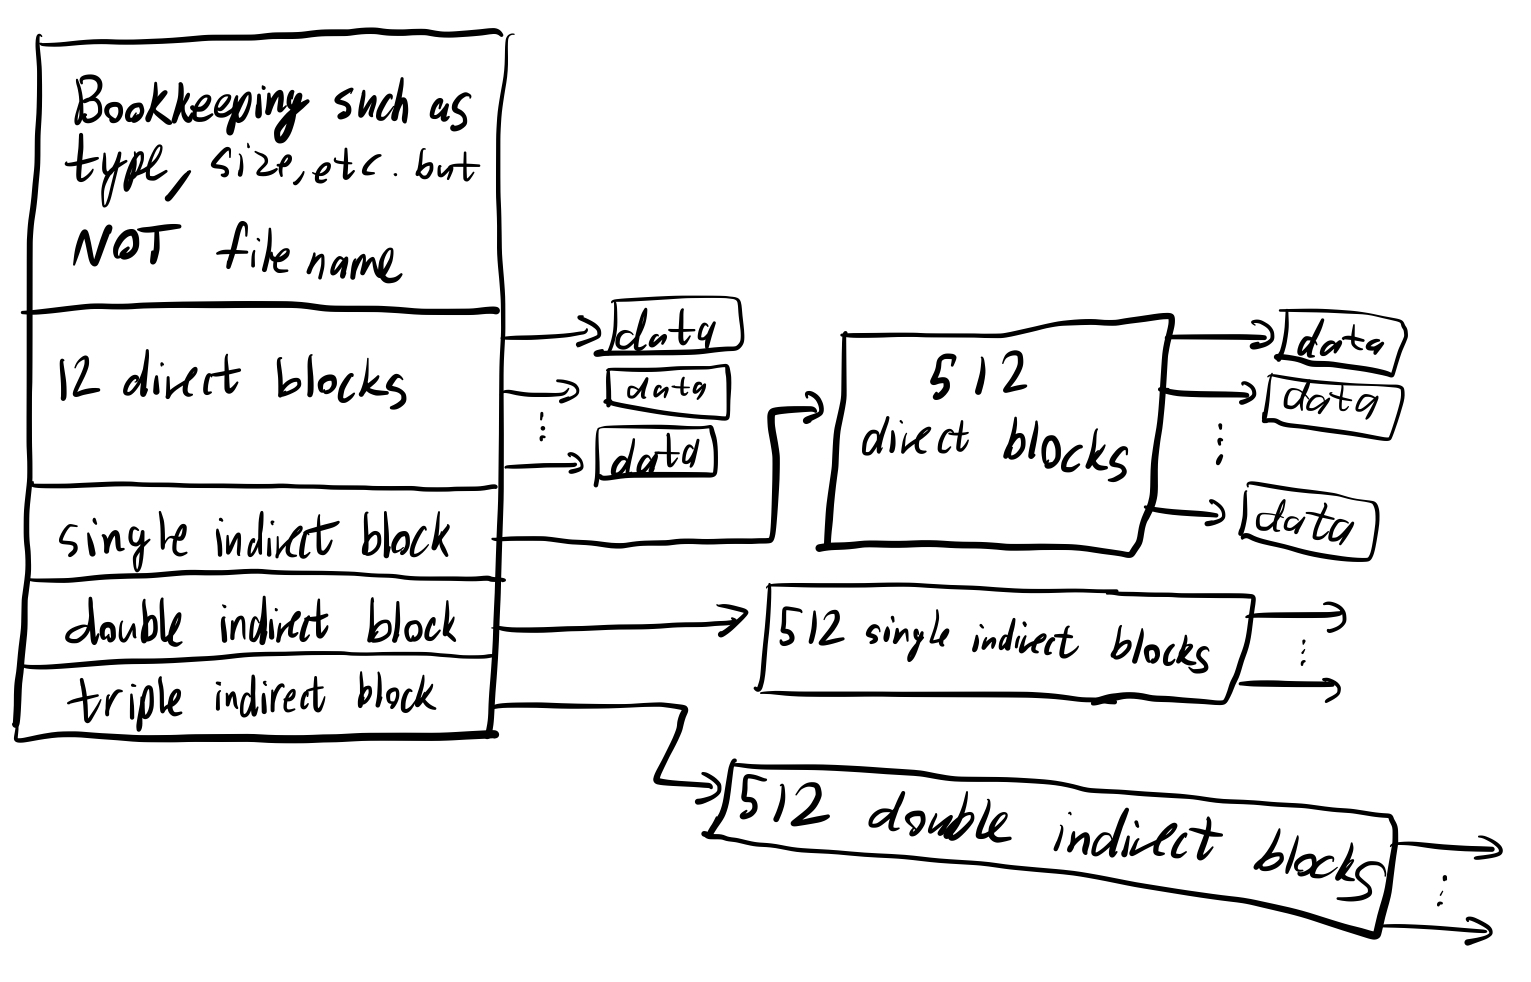
\includegraphics[scale=0.25]{2b.jpg}
        \item \begin{itemize}
            \item 1 triple indirect block $=>$ 512 double indirect blocks $=>$ 512 + 1 = 513 double indirect blocks in total
            \item 513 double indirect blocks $=>$ 513 * 512 = 262656 single indirect blocks $=>$ 262656 + 1 = 262657 single indirect blocks in total
            \item 262657 single indirect blocks $=>$ 262657 * 512 = 134480384 direct blocks $=>$ 134480384 + 12 = 134480396 direct blocks in total
            \item 134480396 direct blocks $\times$ 512 bytes per block $\approx$ 64.1 GB 
        \end{itemize}
        
        

    \end{enumerate}
    \item \begin{enumerate}
        \item TODO
        \item This only achieves the intended purpose to a certain extent. It mitigates against accidental file deletions as if a file is deleted on a filesystem but exists on a previous snapshot, the hard link count will not be zero so the file will not be deleted entirely. However it does not provide a backup to edits. The hard links all point to the same file on disk, so if a file is edited, all hard links to it (i.e. all snapshots) point to the edited version. The major advantage of this method is that it saves on disk space as each file isn't duplicated every day (which would take huge amounts of space) and new hard links are just created. A major disadvantage, as mentioned, is that this does not mitigate against accidental file edits. Also, once a day may not be frequent enough and doing this once every 5 minutes, for example, may not be feasible as it may take longer than 5 minutes to recursively copy all the files (or even longer than a day).
    \end{enumerate}
    \item The formula Unix uses for priority scheduling of jobs gives jobs which previously used less CPU time higher priority, i.e. I/O-intensive jobs.
    \item Unix inodes contain the following information:\\
    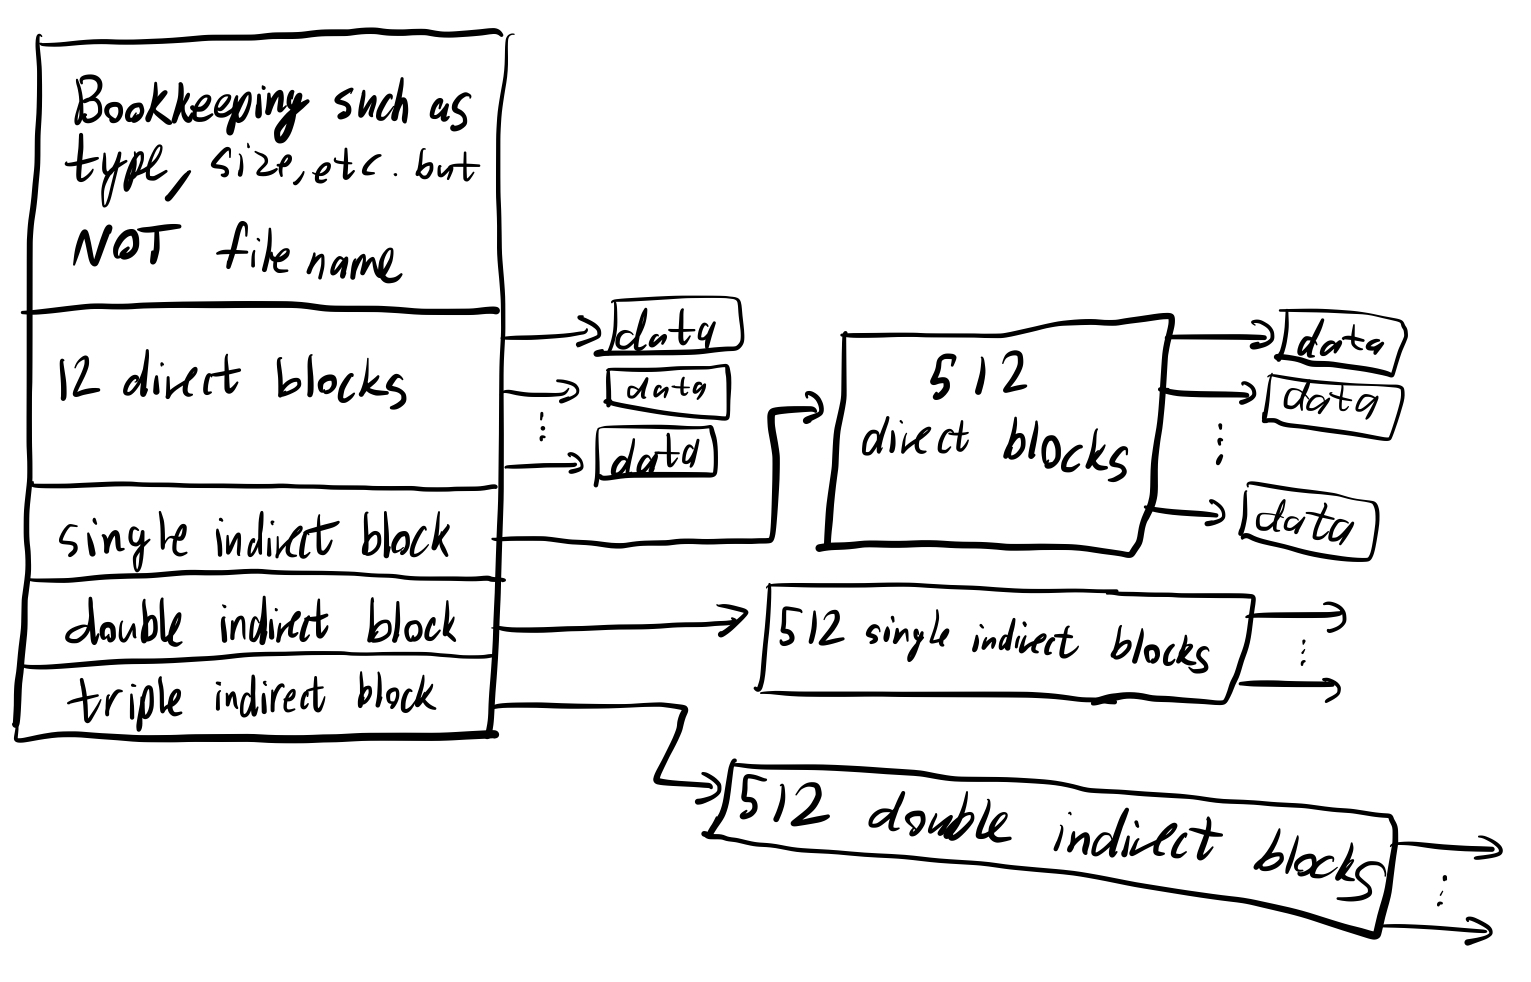
\includegraphics[scale=0.25]{2b.jpg}\\
    If all the blocks were direct blocks then every time you load an inode you would have toload all addresses of all data of the inode, while with indirect blocks you can load them in as needed.
    \item The shell is just a process. As seen in the diagram below, it consists of an infinite loop:
    \begin{enumerate}[1.]
        \item issues prompt (write)
        \item gets input from command line (read)
        \item creates child process (fork)
        \begin{itemize}
            \item if in foreground, waits for completion of fork
            \item if in background, goes back to write
        \end{itemize}
        \item executes program (execve)
        \item becomes a zombie process and terminates (exit)
    \end{enumerate}
    TODO DIAGRAM HERE
\end{enumerate}

\section{Tripos Question 2012/II/4}
\begin{enumerate}[(a)]
    \item \begin{enumerate}[(i)]
        \item Byte 70 would be in the immediate data, so it can be directly accessed, i.e. just one disk block needs to be read.
        \item Each block address is $32=2^5$ bits. There are a total of $1024=2^{10}$ direct block pointers, so there are a total of $2^5$ direct blocks pointed to by the inode. The indirect block pointer points to a block which points to $2^5$ other blocks, i.e. $2^6$ so far (plus another 2040 from the immediate data). Therefore a double indirect is needed. A double indirect block contains $2^5$ indirect blocks. To get to $2^{20}$ we therefore need 4 indirect blocks pointing between them, and a fifth disk read to get the data stored at 2044 in that, i.e. a total of 5 disk block reads.
    \end{enumerate}
    \item Immediate access (1 disk read): $2044$ B\\
    Direct blocks (2 disk reads): $\dfrac{1024}{4} \times 4096 = 1$ MB\\
    Indirect blocks (3 disk reads): $\dfrac{4096}{4} \times 4096 = 4$ MB\\
    $\therefore$ $\text{total} = 6 \text{ MB} + 1020 \text{ B}$
    \item \begin{enumerate}[(i)]
        \item Time of creation is stored in the inode as hard links all refer to the same file on disk and we care about when the content itself was created rather than the rather arbitrary time it was hard linked in the directory.
        \item File name is stored in the directory as the hard link can have different names in different directories.
        \item File access rights are stored in the inode as there is no point in having different access rights in different directories as if a user does not have access rights to the file in one directory but they do in another, there's nothing stopping them from just accessing it from the other directory.
    \end{enumerate}
    \item With this method, reading is very fast as a lot of data is stored directly in the first block and one only has to look at the next byte for the address to the next block. However, writes and file creation are slow as a high degree of fragmentation can occur so empty spaces need to be found.
\end{enumerate}

\section*{Tripos Question 2010/II/4}
\begin{enumerate}[(a)]
    \item \begin{enumerate}[(i)]
        \item The text segment contains the plaintext (uncompiled) code of the process being run. This doesn't change during the process (unless it modifies its own code for some reason).
        \item The data segment contains static variables. This segment grows as more space is allocated for variables.
        \item The stack segment contains the stack of function calls, growing as child processes are created and shrinking as they terminate.
    \end{enumerate}
    \item Only parts (a) and (d) in supervision work.
    \item Only parts (a) and (d) in supervision work.
    \item \begin{enumerate}[(i)]
        \item Requests will be made to the drive when a filesystem request is made to read a file, and when the buffer cache would like to write dirty blocks back to disk.
        \item When an interrupt occurs, the driver needs to find the process that asked for I/O with the disk and enter it back into the job queue.
        \item We need to do things like waiting for a certain number of requests or a certain amount of time before writing dirty data to disk rather than doing it every time a block is modified so that the number of writes don't get too large.
    \end{enumerate}
\end{enumerate}

\end{document}
